\begin{thm}{160}{\hosi 7}{京大 (2014)}
 $xy$平面の第一象限において、原点Oを中心とする円$C_1$と、$C_2: y=\dfrac{1}{x} (0<x)$ が2点A, Bで交わっている。点Aにおける$y=\dfrac{1}{x}$の接線と直線OAのなす角が$\dfrac{\pi}{6}$であるとき、$C_1$と$C_2$で囲まれた部分の面積を求めよ。
\end{thm}

2曲線$C_1$, $C_2$はともに直線$y=x$に関して対称なので、2点A, Bも直線$y=x$に関して対称である。ゆえに点Aは第一象限のうちの$y\le x$の範囲にあるとして一般性を失わない。

円$C_1$の半径を$r$としてA$(r\cos\theta, r\sin\theta)$とおく (ただし$0<\theta<\dfrac{\pi}{4}$)。直線OAの傾きは$\tan\theta$となる。$\theta$の範囲から、$0\tan\theta<1$である。

点Aは曲線$C_2$上の点だから、
\[ r\sin\theta=\frac{1}{r\cos\theta} \,\dou\, r^2\sin\theta\cos\theta=1 \]
が成り立つ。

曲線$C_2$において、$y'=-\dfrac{1}{x^2}$より、点Aにおける$C_2$の接線の傾きは$-\dfrac{1}{r^2\cos^2\theta}$である。ここで、
\[ r^2\cos^2\theta=r^2\cos\theta\sin\theta\frac{\cos\theta}{\sin\theta}=1\cdot\frac{1}{\tan\theta}=\frac{1}{\tan\theta} \]
となるから、この接線の傾きは$-\tan\theta$と書き直せる。したがって、この接線が$x$軸となす角を0から$\dfrac{\pi}{2}$の範囲で考えると、これは$\theta$に等しいことがわかる。これと$0<\theta<\dfrac{\pi}{4}$を踏まえて、点Aにおける$C_2$の接線と直線OAのなす角は$2\theta$であることがわかる。さらにこれが$\dfrac{\pi}{6}$に等しいから、$\theta=\dfrac{\pi}{12}$と求まった。加えて
\[ 1=r^2\cos\theta\sin\theta=r^2\frac{1}{2}\sin2\theta=r^2\frac{1}{2}\sin\frac{\pi}{6}=\frac{r^2}{4} \]
によって$r^2=4$を得る。\footnote{ここまでの議論は、はてなブログを参考にしつつ、編者が改訂を行っています。}

\begin{figure}[H]
 \centering
 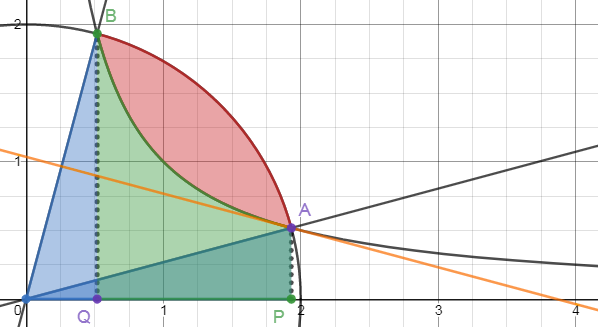
\includegraphics[width=0.7\linewidth]{../problems/Q_160/A_160.png}
\end{figure}
点A, Bから$x$軸におろした垂線の足をP, Qとする。2曲線$C_1$, $C_2$で囲まれた部分の面積は、
\[ \text{扇形}\mr{OAB} + \triangle\mr{OAP}-\triangle\mr{OBQ}- (\text{上図緑領域}) \]
によって求められる。ここで$y=x$についての対称性から、直線OBと$y$軸のなす角は$\theta=\dfrac{\pi}{12}$に等しい。よって点Bの$x$座標は$r\sin\theta$であり、また$\angle\mr{AOB}=\dfrac{\pi}{3}$。さらに、$\angle\mr{BOQ}=\angle\mr{OAP}$であり、BO=OAとあわせれば$\triangle\mr{OAP}\equiv\triangle\mr{BOQ}$が成り立つから面積も等しい。これらを用いて求める面積は、
\begin{align*}
 &\frac{r^2}{2}\frac{\pi}{3}-\int_{r\sin\theta}^{r\cos\theta}\!\frac{1}{x} \,dx \\
 =& \frac{2}{3}\pi-\bigl[\log x\bigr]_{r\sin\theta}^{r\cos\theta} = \frac{2}{3}\pi -\log\left(\frac{1}{\tan\theta}\right)
\end{align*}
で求められる。さて、
\[ \frac{1}{\tan\theta}=\frac{1}{\tan\frac{\pi}{12}}=\sqrt{\frac{1+\cos\frac{\pi}{6}}{1-\cos\frac{\pi}{6}}}=2+\sqrt{3} \]
であるから、求める面積は、$\dfrac{2}{3}\pi-\log{(2+\sqrt{3})}$